%% 
%% Copyright 2019-2020 Elsevier Ltd
%% 
%% This file is part of the 'CAS Bundle'.
%% --------------------------------------
%% 
%% It may be distributed under the conditions of the LaTeX Project Public
%% License, either version 1.2 of this license or (at your option) any
%% later version.  The latest version of this license is in
%%    http://www.latex-project.org/lppl.txt
%% and version 1.2 or later is part of all distributions of LaTeX
%% version 1999/12/01 or later.
%% 
%% The list of all files belonging to the 'CAS Bundle' is
%% given in the file `manifest.txt'.
%% 
%% Template article for cas-dc documentclass for 
%% double column output.

%\documentclass[a4paper,fleqn,longmktitle]{cas-dc}
\documentclass[a4paper,fleqn]{cas-dc}

\usepackage[square,numbers]{natbib}
\usepackage[flushleft]{threeparttable}
\usepackage{makecell}
\usepackage{stfloats}

%%%Author definitions

%%%


\begin{document}
\let\WriteBookmarks\relax
\def\floatpagepagefraction{1}
\def\textpagefraction{.001}

% Short title
\shorttitle{BertNup: A transformer-based model for nucleosome positioning prediction}

% Short author
\shortauthors{Hiep et al.}

% Main title of the paper
\title [mode = title]{BertNup: A transformer-based model for nucleosome positioning prediction}                      
% Title footnote mark
% eg: \tnotemark[1]


% Title footnote 1.
% eg: \tnotetext[1]{Title footnote text}
% \tnotetext[<tnote number>]{<tnote text>} 

% First author
%
% Options: Use if required
% eg: \author[1,3]{Author Name}[type=editor,
%       style=chinese,
%       auid=000,
%       bioid=1,
%       prefix=Sir,
%       orcid=0000-0000-0000-0000,
%       facebook=<facebook id>,
%       twitter=<twitter id>,
%       linkedin=<linkedin id>,
%       gplus=<gplus id>]
\author[1]{Hiep Hoang Dang}
% Footnote of the first author
%\fnmark[1]

% Email id of the first author
\ead{dhoanghiep1998@gmail.com}
%  Credit authorship
%\credit{Conceptualization of this study, Methodology, Software}

% Address/affiliation
\affiliation[1]{organization={Vietnam National University Ho Chi Minh City - University of Science},
    addressline={227, Nguyen Van Cu Street, District 5}, 
    city={Ho Chi Minh City},
    country={Vietnam}}

% Second author
\author[1,2]{Son Thanh Huynh}
\ead{huynhthanh98vn@gmail.com}
\affiliation[2]{organization={AISIA Research Lab},
    % addressline={}, 
    city={Ho Chi Minh City},
    % citysep={}, % Uncomment if no comma needed between city and postcode 
    country={Vietnam}}

% Third author
\author[1,2]{Binh Thanh Nguyen}
% Corresponding author indication
\cormark[1]
\ead{ngtbinh@hcmus.edu.vn}
% Address/affiliation

% Corresponding author text
\cortext[cor1]{Corresponding author}


% Here goes the abstract
\begin{abstract}
Deciphering the regulatory landscape of nucleosome positioning is key to unlocking the intricate mechanisms governing gene expression and chromatin structure. In this study, we introduce BertNup, a novel tool for nucleosome positioning prediction that exclusively employs DNA sequence information. Harnessing the power of the state-of-the-art transformer-based models, pre-trained on a vast array of genomic data, we establish a new standard for human nucleosome positioning prediction, surpassing existing methods. Moreover, our method maintains competitive predictive performance when applied to nucleosome data from various species. Integrating an attention mechanism within the transformer architecture not only enhances the predictive accuracy but also potentially reveals intricate biological information encoded within DNA sequences. This innovation promises to reshape our understanding of gene regulation, chromatin organization, and epigenetic mechanisms across diverse organisms.
\end{abstract}

% Use if graphical abstract is present
% \begin{graphicalabstract}
% \includegraphics{figs/grabs.pdf}
% \end{graphicalabstract}

% Research highlights
% Research highlights
\begin{highlights}
\item Built upon the strength of genomic foundation models, BertNup emerges as a potent predictor of nucleosome positioning.
\item BertNup outperforms previous methods, exhibiting superior predictive capabilities on human data while maintaining competitive results across various species.
\item Attention scores shed light on the mechanism behind BertNup's prediction predictions and hold the potential to uncover novel biological insights.
\end{highlights}
% Keywords
% Each keyword is seperated by \sep
\begin{keywords}
deep learning \sep BERT \sep foundation model \sep genomic \sep nucleosome positioning \sep chromatin structure 
\end{keywords}

\maketitle

\section{Introduction}

The three-billion-base-pair-long human genome is meticulously packaged within the confines of the cell nucleus, a feat achieved through the intricate folding of DNA around histone proteins, forming nucleosomes. Nucleosomes possess a diameter of approximately 10 nm; they serve as the essential building blocks of the chromatin structure in eukaryotic DNA \cite{Kornberg1999}. The central protein core, consisting of eight components referred to as an octamer, includes two sets of histones: H2A, H2B, H3, and H4. Around this structure, roughly 147 DNA base pairs (bp) are tightly coiled, completing about 1.7 turns in a left-handed spiral \cite{Luger1997, Richmond2003}. These 147 bp sequences are called the nucleosome sequence. The DNA segment connecting two adjacent nucleosomes is referred to as a linker. Nucleosomes play a pivotal role in regulating essential cellular processes, such as transcription \cite{Schones2008, Liu2015}, replication \cite{Eaton2010,Liu2017}, and DNA recombination \cite{Smagulova2011, Pulivarthy2016}. The positioning of nucleosomes along the genomic DNA sequence is not random; rather, it is carefully orchestrated and highly influential in determining the accessibility of DNA for various molecular machineries \cite{Kaplan2008}. As such, the precise prediction of nucleosome positioning has emerged as a captivating puzzle at the crossroads of molecular biology, genomics, and computational biology.

Understanding the principles underlying nucleosome positioning has garnered significant attention due to its potential to unravel the hidden regulatory codes embedded within the genome's structure. The positioning of nucleosomes is a dynamic process influenced by many factors, including DNA sequence preferences, histone modifications, DNA-binding proteins, and higher-order chromatin structures \cite{Struhl2013, Segal2009}. Deciphering these intricate relationships poses a substantial challenge, and computational methods have become indispensable tools. In recent years, a wealth of high-throughput experimental techniques, such as MNase-seq \cite{Kaplan2008, Jiang2009}, DNase-seq \cite{Bell2011,Zhong2016}, ChIP-seq \cite{Schones2008}, and ATAC-seq \cite{Schep2015}, have enabled researchers to probe nucleosome positions across entire genomes. However, these experimental methods are often expensive, labor-intensive, and provide a snapshot of nucleosome positioning under specific cellular conditions. Computational prediction models, on the other hand, offer a cost-effective and rapid means to generate genome-wide nucleosome maps and explore how nucleosome positioning varies across different contexts.

Various computational techniques have been proposed to anticipate the arrangement of nucleosomes. For instance, a range of biophysical approaches, utilizing concepts like thermodynamic stability of DNA sequences \cite{Scipioni2009} or deformation energy \cite{Chen2016}, have emerged for nucleosome positioning predictions. Many machine learning (ML)-based strategies for nucleosome positioning have surfaced, including those rooted in hidden Markov models \cite{Xi2010} and support vector machines (SVM). An illustrative example is the iNUC-PseKNC predictor \cite{Guo2014}, which is SVM-based. This predictor initially compiles a feature vector incorporating six local DNA structural attributes, thus creating a representation of a DNA sequence sample. Subsequently, the feature vector is employed as input for an SVM classifier, allowing nucleosome positioning prediction in species like \textit{H. sapiens}, \textit{C. elegans}, and \textit{D. melanogaster}. This method has been proven to surpass prior predictors in terms of prediction accuracy.

However, these ML-oriented methodologies necessitate manual extraction of features from DNA sequences. Fortunately, given the rapid advancement of deep learning (DL) technologies, this constraint can be mitigated by DL, which can autonomously learn feature representations from raw data \cite{LeCun2015}. Several DL-based models have recently been devised for nucleosome positioning prediction, yielding commendable performance outcomes. LeNup \cite{Zhang2018} if the first DL-based nucleosome positioning predictor. This model encodes DNA sequences into one-hot format and uses the Inception network with a gated convolutional neural network (CNN) to extract nucleosome positioning traits from DNA sequences. LeNup showcased superior performance against previous methods, as evaluated through k-fold cross-validation on an identical benchmark dataset. After the introduction of LeNup, a series of DL-based models emerged. Given the remarkable similarity between the structure of DNA sequences and human language, sequential models like long short-term memory (LSTM) and gated recurrent unit (GRU) have been adopted for predicting components within DNA sequences. While DLNN \cite{Gangi2018} exclusively employs LSTM, other models like CORENup \cite{Amato2020}, DeepNup \cite{Zhou2022}, and NP\_CBiR \cite{Han2022} integrate both CNN and RNN components within their frameworks. These advancements have significantly elevated the benchmark for accurate nucleosome positioning prediction.

Despite the significant advancements achieved by deep learning (DL) techniques in predicting nucleosome positioning, there remains space for enhancing predictive accuracy. Recently, the field of genomics has witnessed groundbreaking advancements with the emergence of new foundation models designed specifically for DNA sequences, notably DNABERT-1 \cite{Ji2021}, DNABERT-2 \cite{Zhou2023} and Nucleotide Transformer \cite{DallaTorre2023}. Introduced in 2021, DNABERT-1 revolutionized the genomics domain by incorporating the pre-training and fine-tuning approach. This innovative strategy involves initial pre-training using the human genome dataset, followed by fine-tuning, enabling DNABERT-1 to achieve remarkable state-of-the-art (SOTA) performance in diverse tasks, including promoter prediction, splicing prediction, and transcription factor binding site prediction. DNABERT-2, building upon its successful predecessor, has been augmented through pre-training with genomes from over 100 species and modifications. It excels across 28 tasks in the Genome Understanding Evaluation benchmark. On the other hand, the expansive Nucleotide-transformer model sets new standards with a massive 2.5 billion parameters, pre-trained on 3202 human genomes and 850 genomes from diverse species. Collectively, these models mark a pivotal moment in genomics, empowering researchers with powerful tools to unravel the intricate mysteries of DNA.

This paper examines the efficacy of a publicly accessible foundational model when subjected to fine-tuning for the task of predicting nucleosome positioning. We introduce our proposed model, BertNup, and evaluate its performance against alternative methods using a 10-fold cross-validation approach. BertNup exhibits superior performance compared to alternative models on human data, while consistently maintaining competitive results across various other species. Furthermore, we conduct a more in-depth exploration of BertNup's operational dynamics by probing the insights it acquires during pre-training and fine-tuning. We visualize the attention map embedded within BertNup to elucidate the genomic elements the model potentially learns to differentiate between nucleosome and linker regions. The outcomes of these analyses underscore BertNup's potency in precisely identifying potential nucleosome sequences and uncovering insights encoded within DNA. For those who are interested, the source code for BertNup is accessible at \url{https://github.com/dhoanghiep/BertNup}.

\section{Methods}

The research objectives addressed in this paper encompass:

\begin{enumerate}[1.]
    \item Evaluating the effectiveness of various foundation models when applied to nucleosome positioning prediction.
    \item Comparing transformer-based models with currently established state-of-the-art approaches for nucleosome positioning prediction.
    \item Gaining insight into model predictions by analyzing attention scores.
\end{enumerate}

The subsequent sections will elaborate on the datasets and methodologies employed within this study.

\subsection{Datasets}

Two widely employed benchmark datasets are utilized to assess the performance of methods to predict nucleosome positioning. The primary group of datasets has been sourced from the research paper by Guo et al. \cite{Guo2014}. This group encompasses a diverse range of species, specifically \textit{Homo sapiens}, \textit{Drosophila melanogaster}, and \textit{Caenorhabditis elegans}. Within each species category, this group comprises a collection of nucleosome sequences as well as linker sequences. Nucleosome sequences are designated as positives, while linker sequences serve as negatives. Uniformly, all nucleosome and linker sequences in this group maintain a consistent length of 147 base pairs. The quantification of positive and negative samples for each species can be found in Table \ref{tbl1}. 

\begin{table}[width=\linewidth,cols=4,pos=h]
	\caption{First group of datasets}
	\label{tbl1}
	\begin{tabular*}{\tblwidth}{@{} LCCC @{} }
		\toprule
		& Nucleosome & Linker & Total \\
		\midrule
		\textit{Homo sapiens} & 2,273 & 2,300 & 4,573 \\
		\textit{Caenorhabditis elegans} & 2,567 & 2,608 & 5,175 \\
		\textit{Drosophila melanogaster} & 2,900 & 2,850 & 5,750 \\

		\bottomrule
	\end{tabular*}
\end{table}

The second dataset originates from the research by Liu et al. \cite{Liu2013}. This dataset collection encompasses multiple species but differs from the first group. Specifically, it encompasses sequences derived from \textit{H. sapiens} (human), \textit{D. melanogaster} (fruit fly), and \textit{S. cerevisiae} (yeast). Notably, this set of datasets is more extensive, with the number of sequences being several orders of magnitude larger than those in the initial group. Within the human and fruit fly datasets, sequences are categorized into three classes: largest chromosome (LC), promoter (PM), and 5'UTR exon regions (5U). The yeast dataset comprises two classes: whole genome (WG) and promoter (PM). The refined sequences are detailed in the publication by Amato et al. \cite{Amato2020}. Notably, all processed sequences maintain a uniform length of 147 base pairs, akin to the sequences in the initial dataset. Table \ref{tbl2} provides an overview of the quantities of nucleosome sequences and linker sequences within this dataset.

\begin{table}[width=\linewidth,cols=4,pos=h]
	\begin{threeparttable}
		\caption{Second group of datasets}
		\label{tbl2}
		\begin{tabular*}{\tblwidth}{@{} LCCC @{} }
			\toprule
			& Nucleosome & Linker & Total \\
			\midrule
			HS - LC & 97,209 & 65,563 & 162,772 \\
			HS - PM & 56,404 & 44,639 & 101,043 \\
			HS - 5U & 11,769 & 4,880 & 16,649 \\
			DM - LC & 46,054 & 30,458 & 76,512 \\
			DM - PM & 48,251 & 28,763 & 77,014 \\
			DM - 5U & 4,669 & 2,704 & 7,373 \\
			Y - WG & 39,661 & 4,824 & 44,485 \\		
			Y - PM & 1,880 & 4,463 & 31,836 \\
			\bottomrule
		\end{tabular*}
		\begin{tablenotes}
			\small
			\item HS: \textit{Homo sapiens}, DM: \textit{Drosophila melanogaster}, Y: Yeast - \textit{Saccharomyces cerevisiae} \\ 
			\item LC: sequences from largest chromosome, PM: sequences from promoter regions, 5U: sequences from 5'UTR exon regions, WG: sequences from whole genome 
		\end{tablenotes}
	\end{threeparttable}
\end{table}

\subsection{Pre-trained foundation models}

\begin{table*}[width=2\linewidth,cols=4,pos=h]
	\begin{threeparttable}
		\caption{Publicly available foundation models for genomic data}
		\label{tbl3}
		\begin{tabular*}{\tblwidth}{@{} LCCC @{} }
			\toprule
			\makecell[l]{Pre-trained model} & \makecell{Model size (\# parameters)} & \makecell{Pre-trained data} & DNA sequence tokenizer \\
			\midrule
			BERT-base-cased & 110M & English corpus & Single character tokenizer \\
            DNABERT-1 & 86M & Human genome reference & Overlapping k-mer tokenizer, k $\in [3,4,5,6]$ \\
			DNABERT-2 & 117M & Genomes from 135 species & BPE tokenizer \\
			\makecell[l]{Nucleotide-Transformer\\-500M-human-ref} & 500M & Human genome reference & Non-overlapping 6-mer tokenizer\\
            \makecell[l]{Nucleotide-Transformer\\-500M-1000G} & 500M & 3202 human genomes & Non-overlapping 6-mer tokenizer \\
			\bottomrule
		\end{tabular*}
	\end{threeparttable}
\end{table*}
This study embarks on a comprehensive exploration of the utilization of advanced transformer-based models within the realm of genomic data analysis. The models under scrutiny are outlined in Table \ref{tbl3}. Specifically, the models subjected to testing encompass:

\begin{itemize}
    \item Bidirectional Encoder Representations from Transformers (BERT) \cite{Devlin2019}: Despite undergoing initial pre-training on English text, BERT exhibited impressive adaptability when applied to the genomics field \cite{Le2021, Charoenkwan2021}. Commonly employed approaches utilize BERT as a feature extraction module, transforming DNA sequences into informative representations. Subsequently, prediction can be performed using other machine learning classifiers.
    \item DNABERT \cite{Ji2021}: As the pioneer foundation model pre-trained with human genome DNA sequences, DNABERT has attained unprecedented state-of-the-art performance across various genomic tasks. A central feature of DNABERT-1 revolves around implementing an overlapping k-mer tokenizer, effectively assimilating more intricate contextual information. The authors introduced four pre-trained models, each configured with distinct k values selected from the set \{3, 4, 5, 6\}, thus enhancing versatility and adaptability. In this paper, we denote four versions of DNABERT as: DNABERT-1-3, DNABERT-1-4, DNABERT-1-5, and DNABERT-1-6. This distinction is made to differentiate them from their successor: DNABERT-2.
    \item DNABERT-2 \cite{Zhou2023}: Drawing upon the accomplishments of DNABERT, DNABERT-2 introduces notable enhancements. The pre-training dataset encompasses genomes from more than 135 species, encompassing fungi, protozoa, vertebrates, and bacteria. Additionally, the authors adopt Byte Pair Encoding (BPE) \cite{Sennrich2016}, a widely employed data compression algorithm, replacing the previous k-mer tokenization approach.
    \item Nucleotide Transformer \cite{DallaTorre2023}: Proposed by Dalla-Torre and colleagues, Nucleotide Transformers comprises a sequence of genomic foundation models ranging from 500M to 2500M parameters. Nucleotide Transformers adopted non-overlapping k-mer tokenization, and the largest model was pre-trained on an extensive dataset of genomes spanning 850 species. Our investigation assesses the 500M parameter models within the Nucleotide Transformers family, namely Nucleotide-Transformer-500M-human-ref and Nucleotide-Transformer-500M-1000G. Nucleotide-Transformer-500M-human-ref was pre-trained with GRCh38 human reference genome, and Nucleotide-Transformer-500M-1000G was pre-trained with 3202 human genomes from the 1000 Genome project \cite{ByrskaBishop2021}.
\end{itemize}

These pre-trained models have shown exceptional capabilities in capturing intricate patterns within sequential data of DNA. To tailor these models for the specific task of predicting nucleosome positioning, we conducted fine-tuning on our datasets, treating the DNA sequences as sequential inputs. We processed the DNA sequences by utilizing the designated tokenizer associated with the chosen models.

\subsection{Model fine-tuning details}

We approach the nucleosome prediction problem as a binary classification task, distinguishing between nucleosome sequences and linker sequences. The DNA sequences are converted to numeric vectors by the tokenizer tailored to the chosen foundation models. We introduce two special tokens within this process: [CLS] is appended at the sequence beginning, and [SEP] is appended at the end. The foundation transformer-based model will produce the learned embeddings for each token in the DNA sequence. The entire DNA sequence representation is obtained through the last-layer embedding of the [CLS] token. After pooling using the [CLS] token, we apply a fully connected layer and sigmoid function to generate a final prediction score, falling within the $[0,1]$ range. A predetermined ``threshold" is applied; sequences with a prediction score greater than the threshold are classified as positive or nucleosome sequences, while those below the threshold are classified as negative or linker sequences.

In the experiment to assess the performance of genomic foundation models, we employed the HS - LC dataset. This dataset was partitioned into training, testing, and validation sets in an 8:1:1 ratio, respectively. The models underwent fine-tuning utilizing specific hyperparameters, including a batch size of 32, a learning rate of $2 * 10^{-5}$, a maximum of 10 epochs, and implementing a linear warmup with a linear decay optimizer. For the warmup phase, the number of warmup steps was set to 10\% of the maximum steps. The model with the best performance on the validation set was selected as the final model. Ultimately, the model's performance was evaluated using the designated test set.

We employed both datasets to compare the optimal transformer-based model with alternative methods. A 10-fold cross-validation approach was adopted for model evaluation. Each dataset was partitioned into ten distinct splits while preserving class distribution. During each iteration of the 10-fold cross-validation, one fold was designated as the independent test set, another as the development set for model validation, and the remaining eight folds were utilized for training purposes.

Hyperparameters employed encompassed a batch size of 32, a learning rate set at $2 * 10^{-5}$, a maximum of 10 epochs, and integration of a linear warmup of 40 steps with a linear decay optimizer. Within each epoch, validation was performed ten times. Additionally, a mechanism of early stopping was implemented: if the model's loss does not decrease after ten consecutive validation steps, the training process will be terminated. Subsequently, the best-performing model will be evaluated through the test split. The final evaluation metrics will be recorded. A mean score was computed across the ten iterations for all the metrics to consolidate the outcomes.


\subsection{Evaluation metrics}
Several evaluation metrics are used to compare the performance of the model. Those are $Sensitivity$, $Specificity$, Accuracy ($ACC$), \textit{F1 score}, Matthews correlation coefficient ($MCC$) and the area under receiver operating characteristic curve ($AUC$). These assessment metrics are widely used within the field of bioinformatics. They were also employed in the previous studies on nucleosome positioning prediction \cite{Zhang2018, Amato2020, Han2022}. 

The $Sensitivity \in [0,1]$ represents the ratio of correctly predicted positive samples (nucleosome sequences) to the total positive. The $Specificity \in [0,1]$ represents the ratio of correctly predicted samples (linker sequences) to the total negative samples. The metric $ACC \in [0,1]$ represents the ratio of both correctly predicted positive and negative samples to the entire dataset. \textit{F1 score} $\in [0,1]$, combines precision and recall to provide an overall assessment of classification performance in case of imbalanced data. The $MCC$ metric $\in [-1, 1]$ also serves as a measure of prediction quality for a binary classifier. The first five metrics are defined as below:

$$ Sensitivity = \frac{T_p}{T_p + F_n} $$
$$ Specificity = \frac {T_n}{T_n + F_p} $$
$$ ACC = \frac{T_p + T_n}{T_p + F_n + T_n + F_p} $$
$$ \textit{F1 score} = \frac{2 * T_p}{2* T_p + F_p + F_n} $$
$$ MCC = \frac{T_p * T_n - F_p * F_n}{\sqrt{(T_n + F_n) * (T_n + F_p) * (T_p + F_n) * (T_p + F_p)}} $$
where $T_p$ is true-positive, $F_p$ is false positive, $T_n$ is true negative and $F_n$ is false-negative. The classification threshold of 0.5 was used to compute these metrics.

We also use the metric area under the receiver operating characteristic curve ($AUC$) to quantify the model's performance. The $AUC$ value is obtained by computing the area under the curve of the receiver operating characteristic, which is generated by plotting the $Sensitivity$ metric on the X-axis and the $1 - Specificity$ metric on the Y-axis using various classification thresholds. A higher AUC value, approaching 1, indicates superior model performance.

We meticulously extracted evaluation metrics from the source papers corresponding to the respective methods to facilitate a meaningful comparison with other methods. This process ensures that the assessment of our proposed method remains grounded in the established context and benchmarks provided by the existing literature.

\subsection{Attention scores visualization}

DNABERT-viz\cite{Ji2021} was used to directly visualize the significant region in the input sequence. To elaborate, we consider the vector $q^*$ with dimension $d$; this is the query vector of the [CLS] token specialized symbol added at the sequence's beginning for final classification. We denote $k_j$ as the key vector for the $j$-th k-mer token, $j \in \{1,...J\}$, where J represents the number of tokens in the input sequence. Consequently, the attention score for each embedded k-mer token across all attention heads H is the summation of softmax values: 

$$ \alpha_j=\sum_{h=1}^{H}\frac{\exp(q^{\ast T}k_j/\sqrt d)}{\sum_{l=1}^{J}{\exp(q^{\ast T}k_l/\sqrt d)}} $$

In essence, this process involves extracting the attention of the "entire sequence" concerning k-mer subsequences and utilizing it as a measure of significance. To transition from the k-mer attention score to the individual nucleotide level, we calculated the average scores for all k-mers that include a particular nucleotide. Subsequently, heatmaps representing the attention of each individual nucleotide are generated, allowing for intuitive and direct visualization of their importance.
\section{Result}
\subsection{Transformer-based model performance on nucleosome positioning prediction}
\begin{table*}[width=2\linewidth,cols=7,pos=h]
	\caption{Nucleosome prediction performance of different transformer-based models - Dataset HS - LC}
	\label{tbl4}
	\begin{tabular*}{\tblwidth}{@{} L|cccccc@{} }
		\toprule
		& \textbf{Specificity} & \textbf{Sensitivity} & \textbf{Accuracy} & \textbf{F1 score} & \textbf{MCC} & \textbf{AUC}\\
		\hline
		\textbf{DNABERT-1-3} & \textbf{0.8238} & 0.9632 &\textbf{0.9092} & \textbf{0.9285} & \textbf{0.8085} & \textbf{0.9498} \\
		DNABERT-1-4 & 0.8015 & 0.9748 & 0.9076 & 0.9281 & 0.8068 & 0.9464 \\
		DNABERT-1-5 & 0.7933 & 0.9711 & 0.9022 & 0.9240 & 0.7951 & 0.9452 \\
		DNABERT-1-6 & 0.8050 & 0.9731 & 0.9079 & 0.9283 & 0.8071 & 0.9487\\
		DNABERT-2 & 0.7711 & 0.9392 & 0.8740 & 0.9012 & 0.7325 & 0.9216 \\
		Nucleotide-Transformer-500M-human-ref & 0.7643 & \textbf{0.9777} & 0.8950 & 0.9193 & 0.7817 & 0.9376 \\
		Nucleotide-Transformer-500M-1000G & 0.7832 & 0.9675 & 0.8960 & 0.9193 & 0.7818 & 0.9385 \\ 
		BERT-base & 0.7591 & 0.9480 & 0.8747 & 0.9026 & 0.7349 & 0.9198 \\ 
		\bottomrule
	\end{tabular*}
\end{table*}

In the preliminary stage of our investigation, we assessed the predictive capacities exhibited by a total of eight pre-trained transformer-based models. The aim was to appraise their performance in the context of nucleosome positioning prediction. Given that genomic foundations are typically trained on substantial volumes of human data, we assessed nucleosome position prediction using the HS - LC dataset from the second group of datasets. Our approach involved a fine-tuning process employing a train-test-validation strategy. Upon conducting independent evaluations, a consistent pattern emerged across all eight models: transformer-based architectures manifest a notable proficiency in capturing patterns associated with nucleosome positioning (Table \ref{tbl4}). The BERT-based fine-tuned model demonstrates the lowest predictive performance but still exhibits an AUC as high as 0.9198. Conversely, the remaining seven models designed specifically for genomic data display superior predictive capabilities. This outcome underscores the significance of the pre-training process when dealing with genomic data.

Model size does not appear to play a pivotal role in this task. The highest-performing models include the DNABERT-1 family, despite having the most minor parameter count among the tested models at 86 million. Additionally, there is minimal disparity between the two versions of the Nucleotide Transformer family. Despite Nucleotide-Transformer-500M-1000G being pre-trained on a more diverse range of genomes, this enhancement does not significantly contribute to nucleosome sequence prediction. The performance marginally increased from 0.9376 to 0.9385. Unexpectedly, DNABERT-2 declines its capability for nucleosome prediction when contrasted with its precursor, DNABERT-1. This could be attributed to the alteration in the BPE tokenizer, which may have influenced how the model acquires nucleosome-specific features.

In summary, we have opted to delve deeper into the DNABERT-1 family for further investigation. The models fine-tuned with pre-trained DNABERT-1 weights for nucleosome positioning prediction are denoted as BertNup models. In the subsequent section, we embark on a comprehensive comparison between BertNup and other methods, utilizing the two widely used groups of datasets.

\subsection{BertNup performance on the first group of datasets}
\begin{table*}[width=2.1\linewidth,cols=11,pos=bp]
	\caption{Nucleosome prediction performance of different methods via 10-fold cross-validation for three species of the first group}
	\label{tbl5}
	\begin{tabular*}{\tblwidth}{@{} Lc|ccc|ccc|ccc@{} }
		\toprule
		&  & \multicolumn{3}{c|}{\textbf{\textit{Homo sapiens}}} & \multicolumn{3}{c|}{\textbf{\textit{Caenorhabditis elegans}}} & \multicolumn{3}{c}{\textbf{\textit{Drosophila melanogaster}}}  \\ 
		\cline{3-11}
		\textbf{Model} & \textbf{Architecture} & ACC & MCC & AUC & ACC & MCC & AUC & ACC & MCC & AUC \\
		\hline
		iNuc\_PseKNC \cite{Guo2014} & SVM & 0.8627 & 0.7300 & 0.9250 & 0.8690 & 0.7400 & 0.9350 & 0.7997 & 0.6000 & 0.8740 \\
		Lo Bosco et. al.\cite{LoBosco2017} & CNN & 0.8300 & 0.6660 & 0.9100 & 0.8950 & 0.7950 & 0.9600 & 0.8380 & 0.6800 & 0.9200 \\
		DLNN \cite{Gangi2018}& LSTM & 0.8360 & 0.6810 & 0.9200 & 0.8970 & 0.7990 & 0.9600 & 0.8540 & 0.7100 & 0.9300 \\
		LeNup \cite{Zhang2018}& Inception-style & 0.8730 & 0.7620 & 0.9280 & 0.9120 & 0.8320 & 0.9600 & 0.8750 & 0.7660 & 0.9370 \\
		CORENup \cite{Amato2020}& CNN+LSTM & 0.8810 & 0.7580 & 0.9300 & \textbf{0.9150} &\textbf{0.8350} & 0.9600 & \textbf{0.8820} & \textbf{0.7660} & \textbf{0.9400} \\
		DeepNup \cite{Zhou2022}& CNN+GRU & 0.8705 & 0.7421 & 0.9367 & 0.9076 & 0.8166 & \textbf{0.9603} & 0.8621 & 0.7249 & 0.9347  \\
		NP\_CbiR \cite{Han2022}& CNN+BiRNN & 0.8618 & 0.7284 & 0.9234 & 0.8939 & 0.7924 & 0.9530 & 0.8555 & 0.7119 & 0.9251 \\
		DNABERT-1-3 & BERT & \textbf{0.8911} & \textbf{0.7823} & \textbf{0.9450} & 0.8987 & 0.7980 & 0.9588 & 0.8544 & 0.7091 & 0.9259\\ 
		DNABERT-1-4 & BERT & 0.8889 & 0.7778 & 0.9414 & 0.8881 & 0.7768 & 0.9523 & 0.8363 & 0.6761 & 0.9122\\ 
		DNABERT-1-5 & BERT & 0.8754 & 0.7511 & 0.9355 & 0.8914 & 0.7836 & 0.9550 & 0.8360 & 0.6747 & 0.9138\\ 
		DNABERT-1-6 & BERT & 0.8830 & 0.7661 & 0.9374 & 0.8947 & 0.7899 & 0.9550 & 0.8433 & 0.6878 & 0.9213\\ 
		\bottomrule
	\end{tabular*}
\end{table*}
In the evaluation conducted on the first group, which covers three separate datasets \textit{H. sapiens}, \textit{C. elegans}, and \textit{D. melanogaster}, we compare BertNup with various different methods. Our BertNup models exhibited intriguing performance trends (Table \ref{tbl5}). Particularly is the substantial enhancement in predictive accuracy demonstrated within the human dataset, surpassing the achievements of previous models. Notably, the prior best performer was DeepNup with accuracy (ACC) of 0.8705, Matthews correlation coefficient (MCC) of 0.7421, and area under the curve (AUC) of 0.9367. Based on pre-trained DNABERT-1-3, our optimal model showcased improvements with an increase in ACC by 0.0206, MCC by 0.0401, and AUC by 0.0083. This observation underscores our model's aptitude for capturing intricate nucleosome positioning patterns unique to the human genome.

Conversely, our model's performance displayed divergence when confronted with the nematode and fruit fly datasets. In these scenarios, our model's predictive accuracy fell short of that achieved by established methods. Within the nematode dataset, our optimal model attained an AUC of 0.9588, slightly below the best model's AUC of 0.9603 achieved by DeepNup. Similarly, in the fruit fly dataset, the leading model, CORENup, achieved an AUC of 0.9400, whereas our model's AUC lagged behind by 0.0141. This outcome was anticipated because the pre-trained model for BertNup is DNABERT, which was trained solely on the human genome. The observed variations underscore potential differences in nucleosome positioning dynamics across species, implying species-specific regulatory mechanisms that our model may not fully encapsulate.

These comparative results underscore the nuanced nature of nucleosome positioning and the complex interplay of factors shaping it across different organisms. While our model excels in the context of the human genome, its performance nuances across species warrant further investigation. This investigation could potentially lead to insights into the evolutionarily conserved and divergent elements of nucleosome positioning regulation.

\subsection{BertNup performance on the second group of datasets}
\begin{figure*}
	\centering
	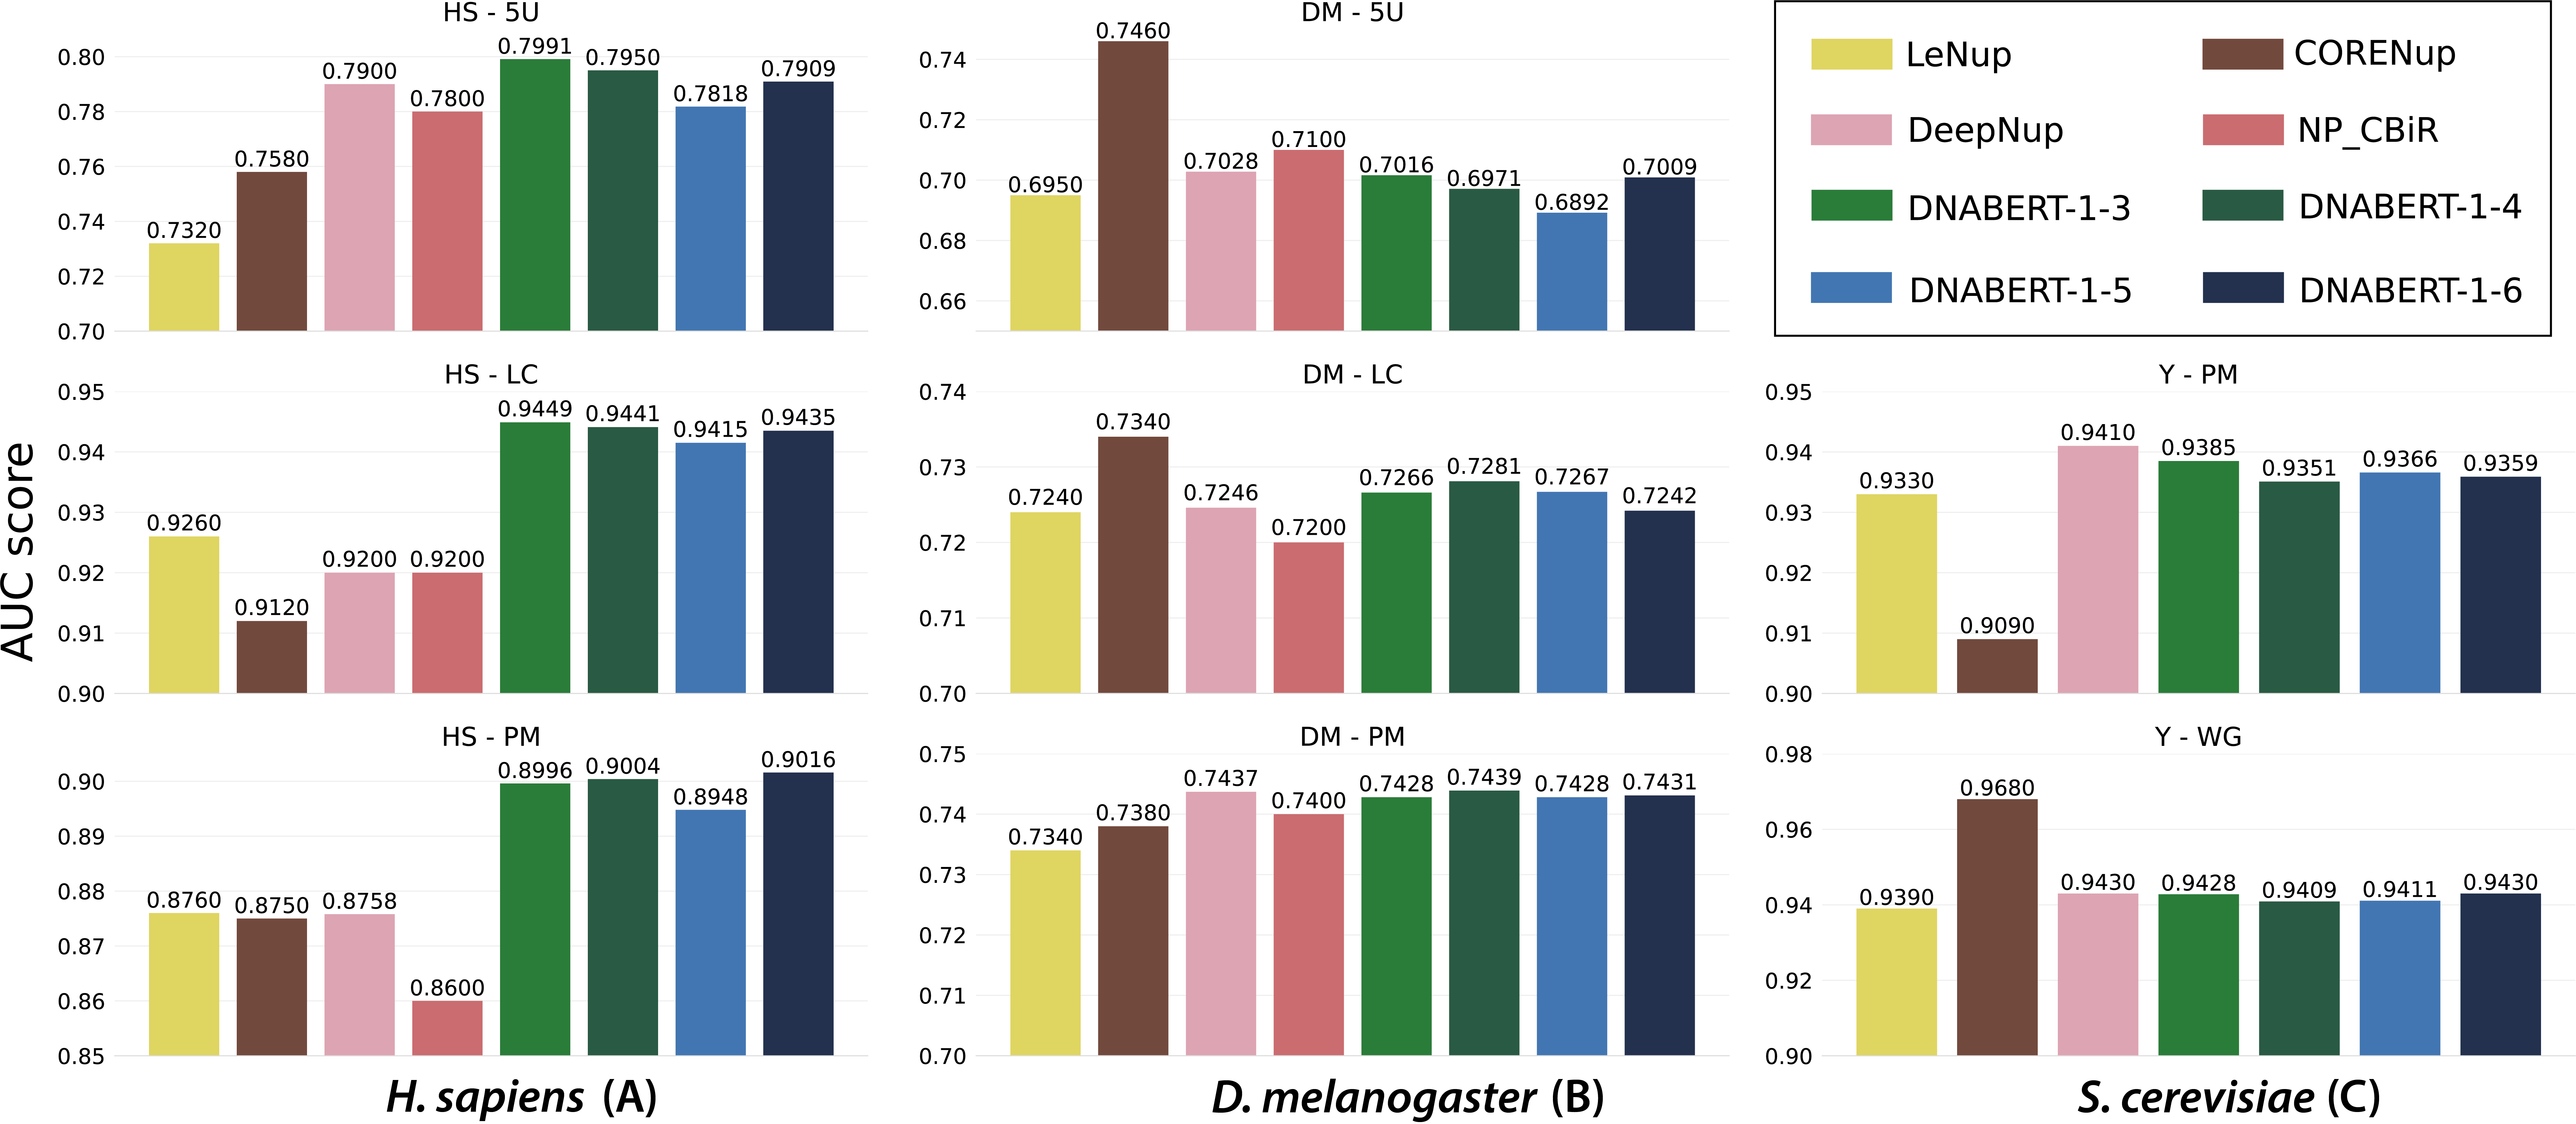
\includegraphics[scale=.25]{figs/fig1.png}
	\caption{Nucleosome prediction performance via 10-fold cross-validation for three species of the second group}
	\label{FIG:1}
\end{figure*}

In the next investigation phase, we turned our attention to a more extensive and diverse group of datasets. Once again, our model's proficiency in nucleosome positioning prediction was evident, particularly within the human genome context (Figure \ref{FIG:1}A).  Outperforming previous approaches, our transformer-based methodology achieved a SOTA outcome on the human datasets. Within the HS - 5U dataset, three out of four versions of BertNup surpassed alternative methods. Notably, in the HS - LC dataset, the BertNup models substantially improved the AUC score, advancing from 0.9260 to 0.9449. Similarly, in the HS - PM dataset, BertNup demonstrated superior performance, with the most significant gain observed from 0.8760 to 0.9016. This accomplishment reaffirms our model's capacity to discern the intricate nuances of nucleosome positioning patterns within the human chromatin landscape.

However, when considering the other species, the performance comparison yielded more nuanced results (Figure \ref{FIG:1}B, C). Our model delivered comparable results to existing models, demonstrating competitive predictive accuracy in these cases. While not surpassing the competition, this consistent performance across diverse organisms underscores the model's adaptability and robustness in capturing species-specific nucleosome positioning patterns.

Intriguingly, when calculating the mean rank performance across all species within this comprehensive dataset, our transformer-based model emerged as the frontrunner (Figure \ref{FIG:2}). The best model is BertNup, fine-tuned from DNABERT-1-3 pre-trained weights, with a mean rank of 3.0. Three of four BertNup models (excluding DNABERT-1-5) exhibit higher ranks than all other methods. This finding signifies a collective dominance across different organisms and reinforces the model's overall predictive capabilities. The highest mean rank showcases the model's generalization potential, suggesting that it excels in capturing the core principles of nucleosome positioning that transcend species boundaries.

\begin{figure}[h]
	\centering
	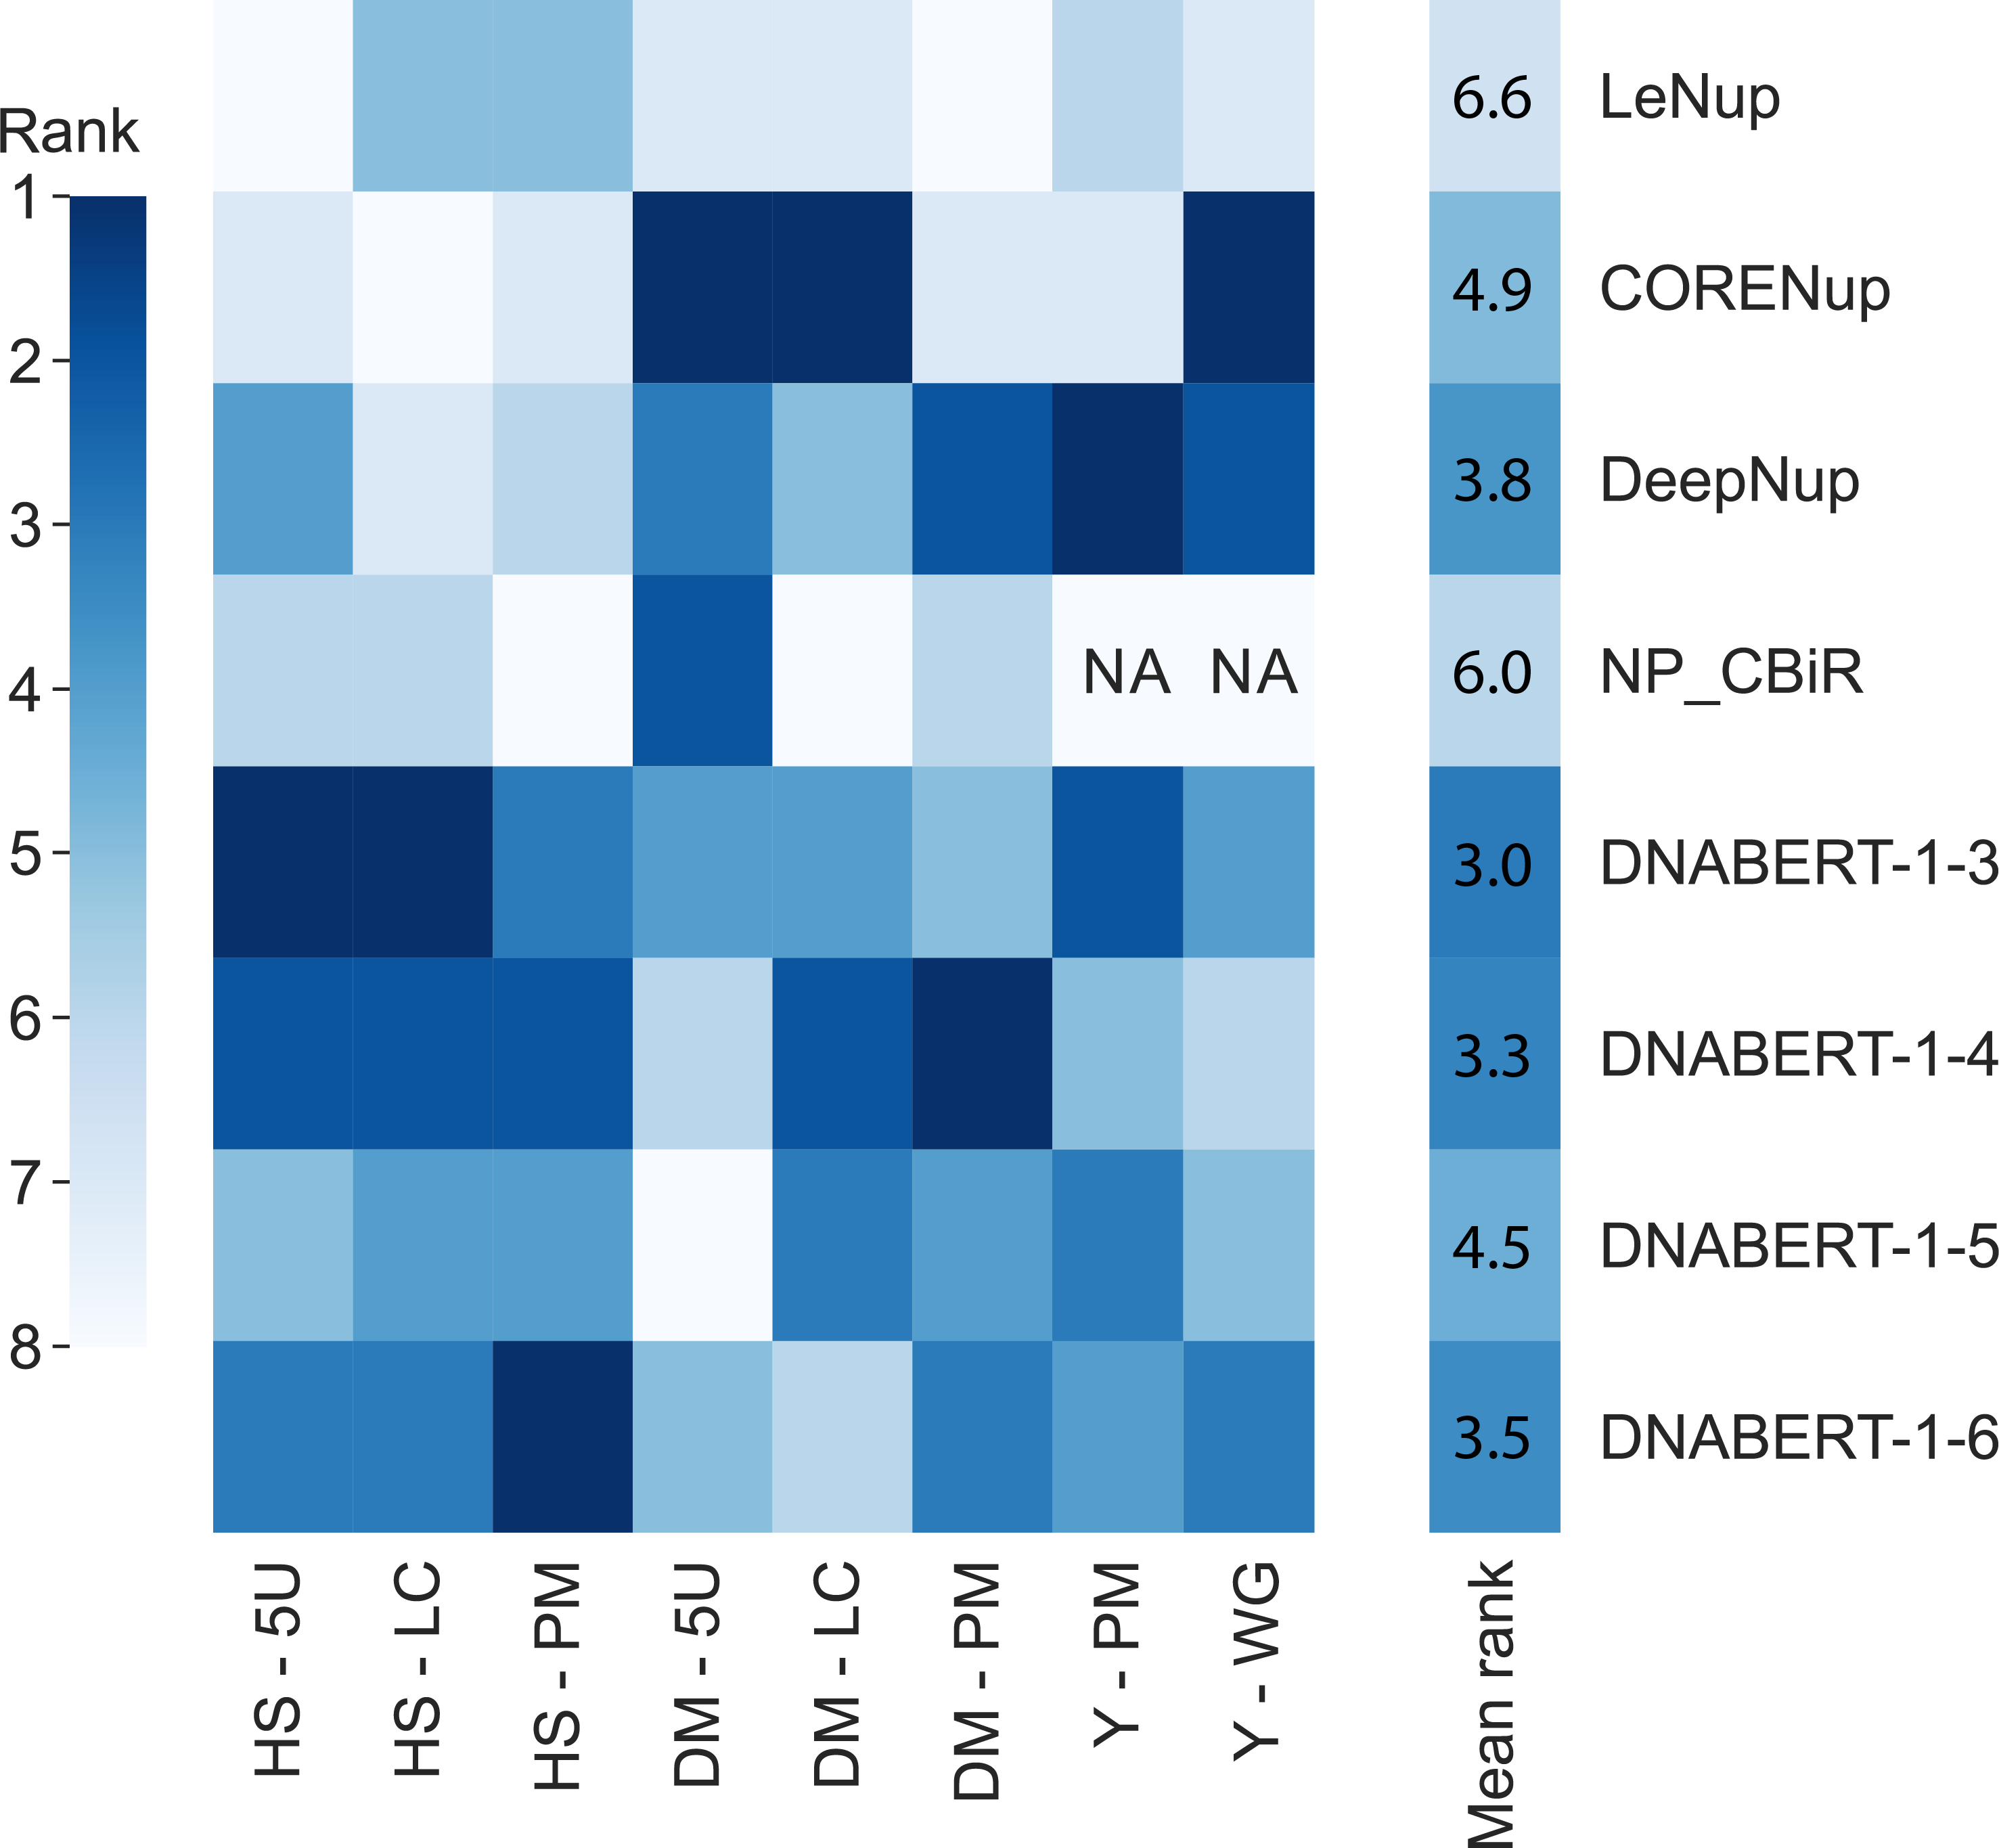
\includegraphics[scale=.27]{figs/fig2.png}
	\caption{Performance ranking within the second group}
	\label{FIG:2}
\end{figure}

These outcomes collectively emphasize the strengths of our transformer-based model, particularly its ability to achieve SOTA results within the human genome and its competitive performance across a spectrum of other organisms. The highest mean rank also underscores the model's overall proficiency and sets a high standard for comparative nucleosome positioning prediction.

\subsection{Gradual comprehension in the pre-training and fine-tuning process}

\begin{figure*}
	\centering
	\includegraphics[scale=.2]{figs/fig3.png}
	\caption{Change of BertNup's attention scores during the process of pre-training and fine-tuning. \textbf{A} Attention landscapes for individuals in the LS - HC dataset. \textbf{B} Average attention scores for each position along the DNA sequence. \textbf{C} Average attention scores for each of the four nucleotides}
	\label{FIG:3}
\end{figure*}

Our goal is to uncover the advantages that BertNup gains through its pre-training process and to shed light on the changes it undergoes during fine-tuning. The inherent attention mechanism within the BERT architecture offers a natural window into the input's significance. We employed DNABERT-viz, a tool derived from the DNABERT framework, to calculate and visualize attention scores. The attention scores are normalized to ensure the sum of attention scores for a sequence equals 1. Consequently, the mean attention score for the nucleosome prediction task becomes $ 1/147 = 0.0068 $, given that the sequences are 147 base pairs in length.

We opted for DNABERT-1-3 as the pre-trained model in this section due to its superior mean rank performance across the eight datasets within the second group. Our focus was on the HS - LC dataset, which is the most comprehensive for human data. We randomly re-initialized all trainable weights in the model architecture to visualize the model with random weights. For the pre-trained weights, we employed the provided weights of DNABERT-1-3. As for the fine-tuned weights, we conducted the fine-tuning process anew by partitioning the dataset into training, testing, and validation subsets using an 8:1:1 ratio. The changes in attention scores were evaluated by assessing the best-fine-tuned model's performance on the test set. The outcomes of this analysis are depicted in Figure \ref{FIG:3}.

The attention scores offer a comprehensive view of how the model's learning process unfolds in nucleosome positioning prediction. This examination encompasses two key dimensions: the evolution of attention scores concerning sequence position and their adaptation based on nucleotide composition. We computed the average attention scores for each position along the sequence, as demonstrated in Figure \ref{FIG:3}B. Average attention scores for each of the four nucleotide types (A, C, G, T) are also calculated and shown in Figure \ref{FIG:3}C.

Before pre-training, the attention scores exhibited a dispersed and fluctuating pattern, underscoring the absence of structured insights within the model's architecture. The attention appeared to be dispersed uniformly across the sequence, with fluctuations converging around an average score for the entire sequence. Similarly, the preference for different nucleotides displayed uniformity, with each of the four nucleotide types (A, C, G, T) maintaining nearly equivalent mean attention scores irrespective of labels.

Following the pre-training phase, a striking transformation emerged in the attention distribution. Scores became conspicuously focused on the initial nucleotides, particularly within the initial five positions. This heightened focus denotes the model's rapid assimilation of sequence-level motifs during the preliminary learning phase. The gradual decline in attention scores beyond this region implies a diminishing emphasis on distal sequence elements—a phenomenon possibly attributed to transformer models' inclination to prioritize local relationships during pretraining. During this phase, a developing preference for different nucleotides became evident, with a slightly elevated attention towards the nucleotide T, registering a mean attention score of 0.0071.

Subsequent fine-tuning marked a significant evolution in attention scores. Attention became more uniformly distributed across the entire sequence, signaling an enhanced grasp of the contextual interplay between nucleotides. Particularly noteworthy was the conspicuous elevation of attention scores within the final 70 nucleotides of the sequence. This heightened sensitivity toward distal regulatory elements or functional motifs positioned towards the sequence's end was observable for both nucleosome and linker sequences.

The nuanced preferences of the fine-tuned models for different nucleotides emerged prominently. Adenine nucleotides were prominently captured by BertNup, boasting the highest mean attention score of 0.0079 for both nucleosome and linker sequences. Thymine nucleotides garnered the second-highest focus. Remarkably, linker sequences exhibited a substantial attention score of 0.0074, while nucleosome sequences remained at an average level of 0.0068. This observation potentially links to nucleosome positioning's strong association with A/T elements—nucleosomes commonly exhibit a periodic distribution of A/T every 10bp \cite{Field2008}, while linker sequences often feature high levels of poly(dA:dT) \cite{Segal_2_2009}.

Our investigation into attention score dynamics provides valuable insights into how the model's understanding evolves across training stages and its attunement to nucleotide-level characteristics. This analysis underscores the model's capacity to identify pivotal sequence features and their potential contributions to nucleosome positioning prediction.

\subsection{The attention head of BertNup reveals genomic-related patterns}
\begin{figure*}
	\centering
	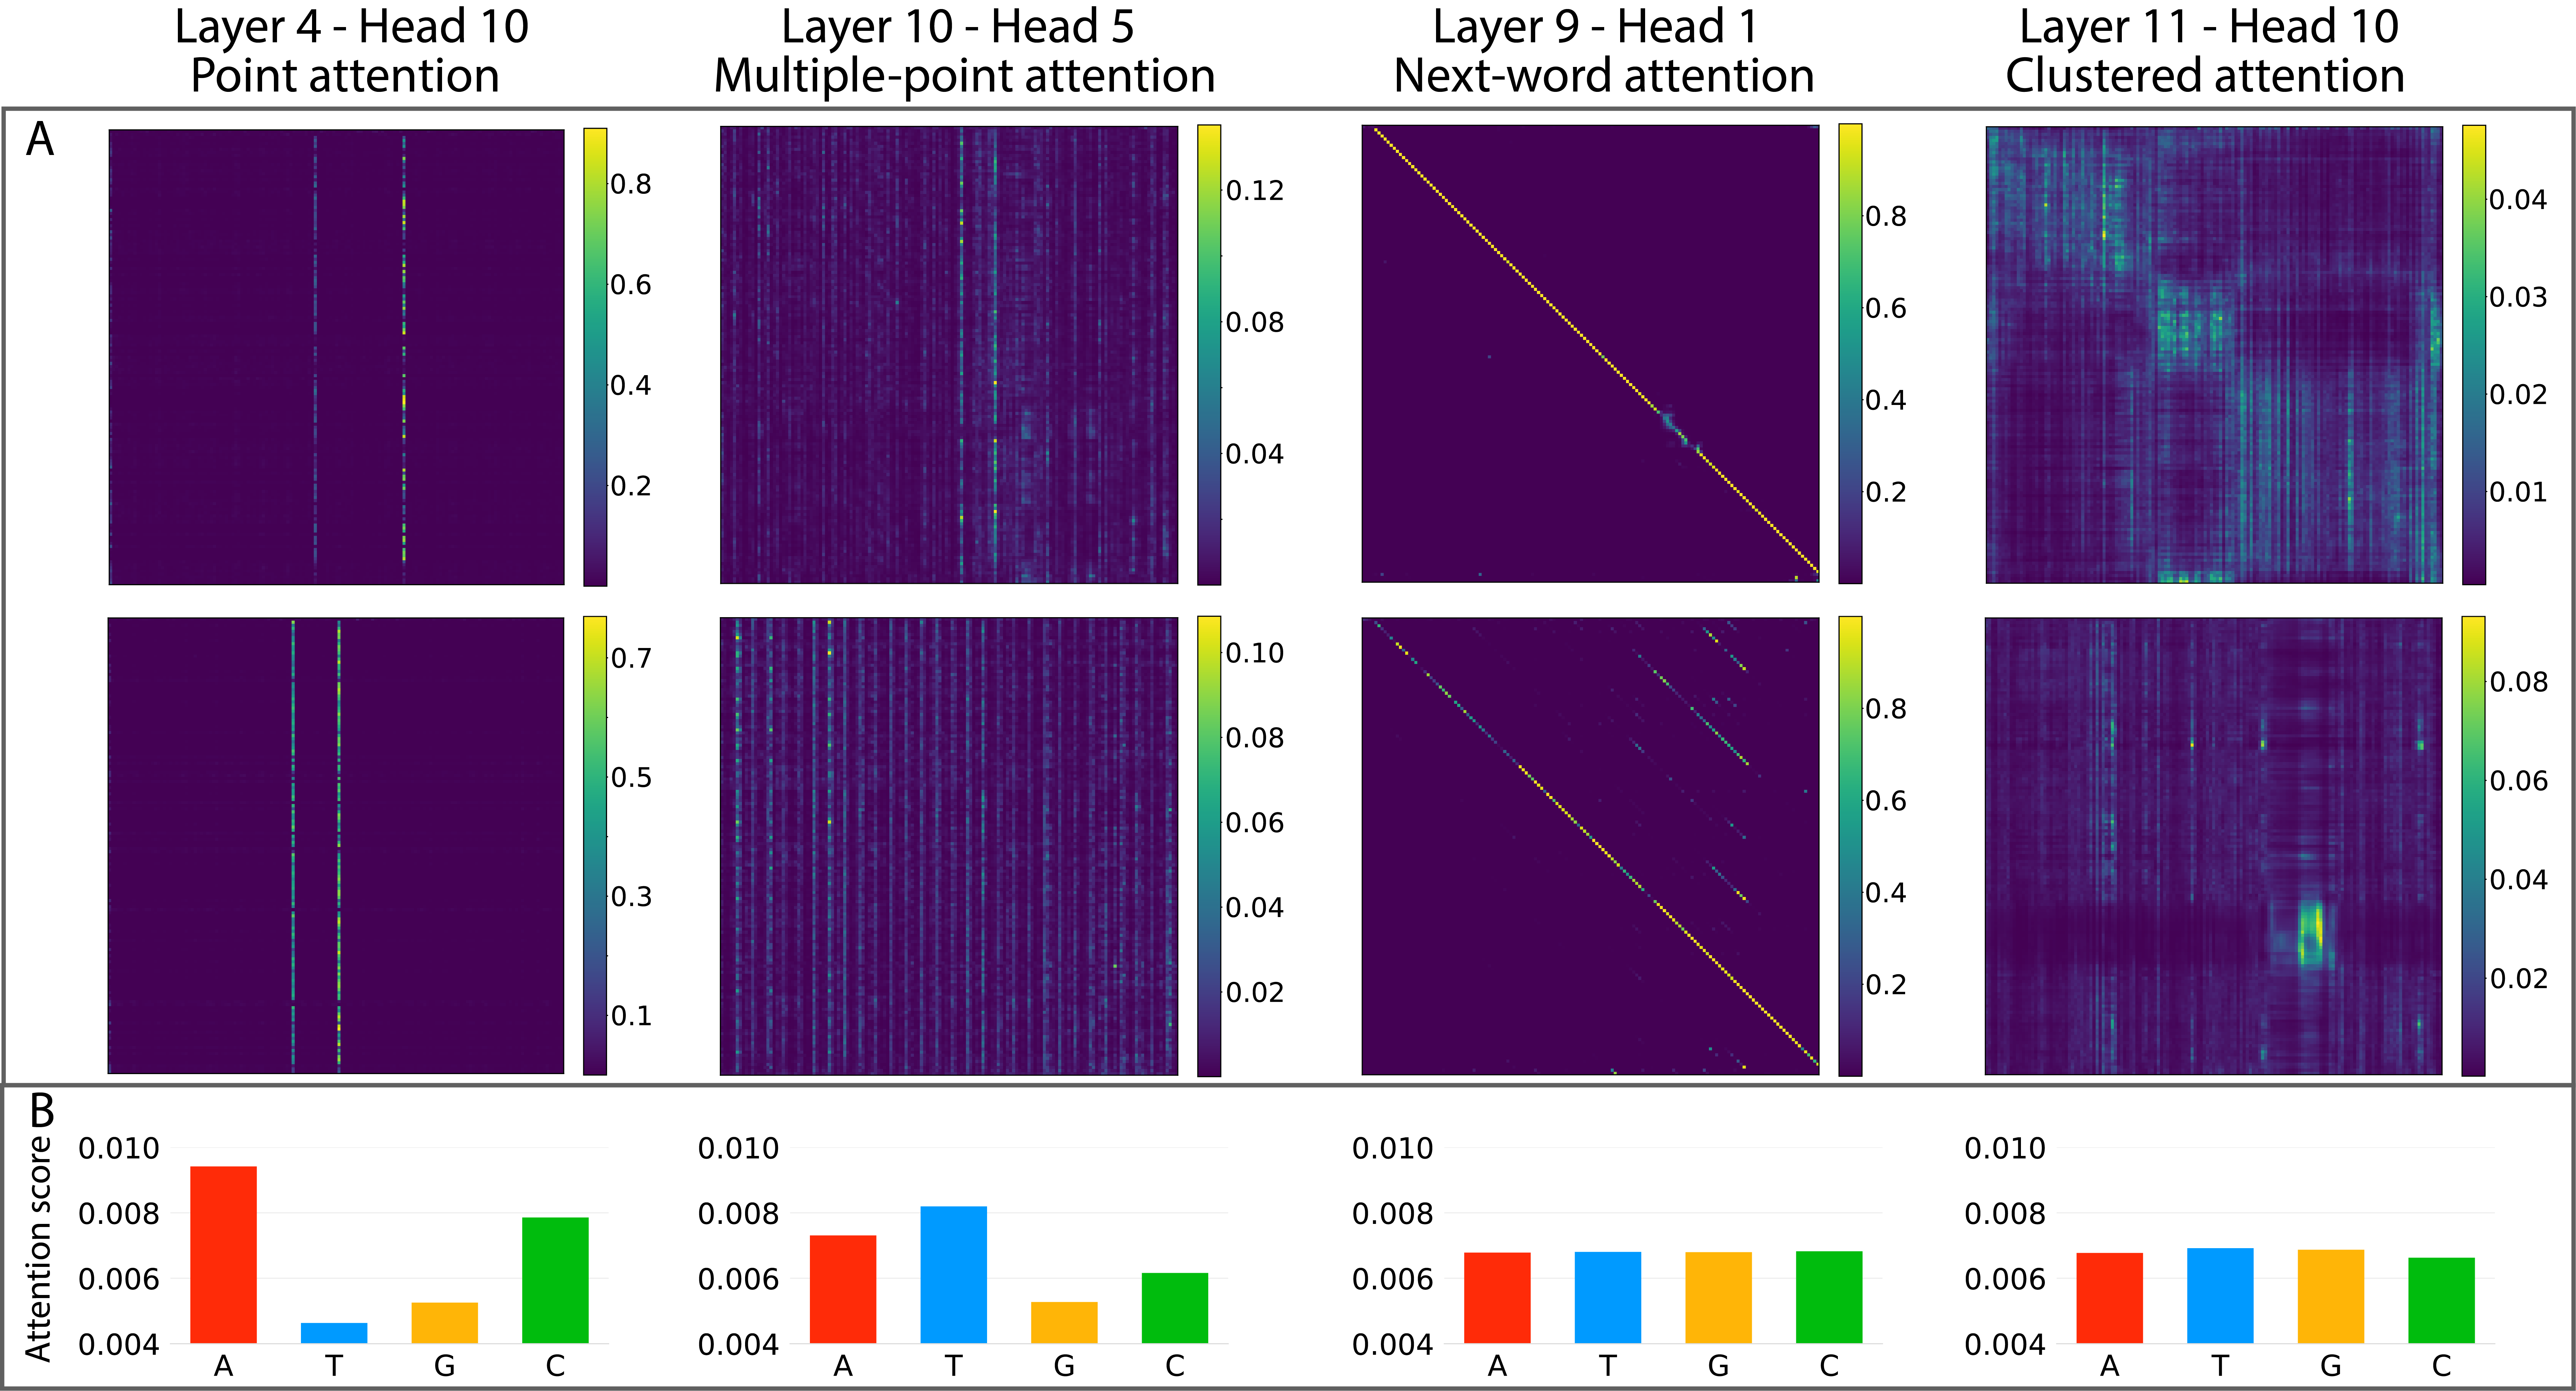
\includegraphics[scale=.22]{figs/fig4.png}
	\caption{Visualization for different groups of attention heads in BertNup. \textbf{A} Attention maps of a specific head for two example DNA sequences. \textbf{B} Average attention scores of a specific head for each of the four nucleotides}
	\label{FIG:4}
\end{figure*}

BERT possesses the capability to capture significant linguistic components through diverse attention heads, such as those focusing on possessive pronouns, preposition-object relationships, and direct object-verb associations \cite{Clark2019}. We embraced a similar notion to uncover attention heads that have learned the underlying genomic structure.

We identified a range of distinct attention patterns upon exploring the attention maps of all 12 layers, each comprising 12 attention heads. Notably, four consistent patterns emerged across the 144 attention heads, potentially harboring encoded genomic elements. These patterns, which we have categorized as single-point attention, multiple-point attention, next-word attention, and clustered attention, served as a basis for uncovering the biological implications inherent in each attention category. Figure \ref{FIG:4}A provides a visual representation of example heads and their attention scores, while Figure \ref{FIG:4}B illustrates the nucleotide preferences associated with attention heads.

\begin{enumerate}[1.]
    \item \textbf{Single-Point Attention}: This attention pattern revealed a remarkable trend in which attention was frequently directed to individual nucleotides. This trend highlights the model's proficiency in identifying critical nucleotide positions pivotal for regulatory interactions. These positions are likely associated with key genomic elements such as transcription factor binding sites or epigenetic markers. For instance, Layer 4 - Head 10 exhibited heightened attention scores for Adenine and Cytosine nucleotides, while Thymine received comparatively lower attention, with a score of 0.0046.

    \item \textbf{Multiple-Point Attention}: Within this specific attention category, the focal point extended to encompass multiple nucleotides distributed periodically. This demonstrated the model's competence in recognizing broader sequence motifs through these patterns of multiple-point attention, which consistently displayed periodic characteristics. While this pattern is generally biased to nucleotide position, noteworthy nucleotide preferences also emerged. For example, in Layer 10 - Head 5, a tendency towards Adenosine and Thymine nucleotides was observed.

    \item \textbf{Next-Word Attention}: Attention scores within this group tended to fall to the immediate neighboring nucleotide or a few nucleotides ahead. This behavior represents the model's anticipation of the next sequential element. No nucleotide preferences were discernible within this attention category.

    \item \textbf{Clustered Attention}: Attention scores within the clustered attention group demonstrated a distinctive tendency to group together, indicating the model's discernment of larger functional units within the sequence. These attention clusters are potentially aligned with functional domains or motifs that influence nucleosome positioning, such as promoter regions or exonic boundaries. Nucleotide preferences were not observed in this attention category.

\end{enumerate}

By categorizing attention patterns into these distinctive groups, we unveiled the intricate foundation upon which the model's understanding of nucleosome positioning dynamics is built. Each attention category offers insights into diverse facets of regulatory biology, ranging from the contributions of individual nucleotides to the orchestration of chromatin architecture by larger functional domains.


\section{Discussion}
Our study has successfully achieved the outlined research objectives:
\begin{enumerate}
    \item Firstly, we thoroughly evaluated the efficacy of different foundation models in the context of nucleosome positioning prediction. Our findings provide valuable insights into the strengths and limitations of these models when applied to this intricate task.
    \item Secondly, we performed a comprehensive comparison between transformer-based models and current state-of-the-art techniques. This analysis shed light on the advancements brought about by transformer-based approaches, demonstrating their competitive edge in nucleosome positioning prediction.
    \item Lastly, our investigation into model predictions through attention scores has provided a deeper understanding of how these models differentiate nucleosome and linker regions. This insight contributes to the interpretability of the models and enhances our grasp of the intricate genomic patterns they capture.
\end{enumerate}


We have embarked on a comprehensive exploration of nucleosome positioning prediction using transformer-based models. Our research sheds light on the dynamic landscape of chromatin architecture and gene regulation, unraveled through the lens of computational biology. As we reflect on the results and implications of our study, three crucial pathways for further investigation emerge:

\textbf{Model Size and Complexity}: The transformer architecture has proven its efficacy across many tasks, thanks to its adaptability and capacity to capture intricate patterns within sequential data. One compelling avenue for future research is the exploration of larger and more complex transformer-based models. While our study has demonstrated the potential of existing models, investigating the impact of increased model size and architectural complexity could yield further advancements in predictive accuracy and deciphering more nuanced regulatory mechanisms. Despite our study's evaluation of Nucleotide Transformers with 500M parameters indicating no significant performance gain, our interest extends to examining the potential of the 2.5B version of Nucleotide Transformers. This pursuit aligns with the general trend in the field of deep learning, where larger models have exhibited the ability to grasp more intricate biological signals, often leading to enhanced predictive performance.

\textbf{Diverse Training Data and Multi-Species Considerations}: Our study has illuminated the capacity of transformer-based models to excel in nucleosome positioning prediction, particularly in the context of the human genome. However, the variability in performance across different species prompts the consideration of diverse training data. Multi-species training, encompassing genomic data from various organisms, presents an exciting opportunity to enhance the model's generalization across species. Investigating how the model's performance evolves when trained on a multi-species dataset could offer insights into conserved and divergent regulatory elements across evolutionarily distinct organisms. This exploration may facilitate the discovery of cross-species regulatory motifs, contributing to our understanding of the evolutionary dynamics underlying nucleosome positioning.

\textbf{Attention Heads for Unraveling Biological Structure}: Our initial investigation into attention scores and the distinct categories of attention heads has unveiled intriguing insights into the model's comprehension of the DNA sequence. However, an even deeper dive into the attention heads themselves holds substantial promise. Exploring individual attention heads and their patterns could potentially reveal finer-grained structural and functional details encoded in the DNA sequence. This avenue aligns with recent trends in explainable AI, where the interpretability of neural network decisions is gaining importance. Unraveling the biological structure embedded in attention heads could bridge the gap between computational predictions and experimentally observed biological phenomena.


\section{Conclusion}
In this research, we conducted a comprehensive exploration of nucleosome positioning prediction using state-of-the-art transformer-based models. Our investigation revealed the models' potential, versatility, and limitations in deciphering nucleosome positioning complexities. Our novel model, BertNup, exhibited impressive performance on human data and competitive results with yeast, fruit fly, and nematode data. We assessed various models and noted distinct performance patterns across diverse species datasets, underscoring the impact of species-specific regulatory mechanisms.

Analyzing attention scores across pre-training and fine-tuning stages, we observed a shift from random attention to targeted regions, followed by a more comprehensive understanding of the entire sequence. Notably, through different processes and training, nucleotide preferences gradually favored A and T in predicting nucleosome sequences. Categorizing attention heads into distinct patterns—single-point, multiple-point, next-word, and clustered—revealed biological insights in DNA sequences.

Looking ahead, future research directions emerge. Exploring larger, complex models could enhance predictive accuracy and pattern detection. Utilizing diverse training data across species might reveal conserved and divergent regulatory motifs. Investigating attention mechanisms' nuances through attention head analysis could bridge computational predictions with biological reality.

Our study highlights transformer-based models' transformative potential in unraveling nucleosome positioning regulations. These models bridge computational biology and genomics, shedding light on chromatin structure and gene regulation. Moving ahead, our insights promise refined predictions, deeper biological understanding, and enriched knowledge of fundamental life principles.



%% Loading bibliography style file
\bibliographystyle{model1-num-names}
%\bibliographystyle{cas-model2-names}

% Loading bibliography database
\bibliography{cas-refs}


\end{document}

